\section{Metodologia Numérica}

\begin{frame}
    \begin{exampleblock}{Metodologia Numérica}
        \begin{itemize}
            \item Método dos Volumes Finitos;
            \item OpenFOAM + cfMesh;
            \item Método VOF;
            \item Modelo bi-viscoso;
            \item interFoam solver;
            \item Automatização Python e Bash.
        \end{itemize}
    \end{exampleblock}
\end{frame}

% \begin{frame}{Método VOF}
%     O método Volume de Fluido, no inglês \textit{Volume of Fluid} (VOF), é usado para capturar a superfície livre do escoamento. A dependência temporal da fase $\alpha$, para um problema bidimensional, é governada pela Eq.~\ref{eq:alpha_phase}.

%     \begin{equation} \label{eq:alpha_phase}
%         \partialderiv{\alpha}{t} + u \partialderiv{\alpha}{x} + v \partialderiv{\alpha}{y} = 0
%     \end{equation}

% \end{frame}

\begin{frame}{Método VOF} 
    \centering
    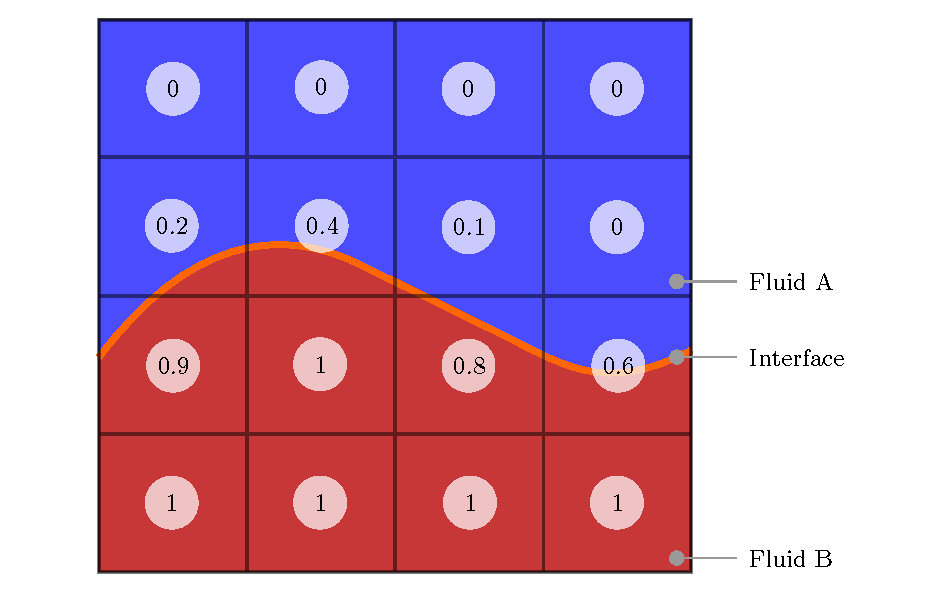
\includegraphics[width=0.68\textwidth]{images/vof.pdf}
    \captionof{figure}{Diagrama esquemático com o valor da fase $\alpha$ no respectivo volume finito.}
\end{frame}

\begin{frame}{Modelo bi-viscoso}
    Para baixas taxas de deformação, o material é modelado como um fluido de alta viscosidade, com valor constante $\eta_0$. Equação~\ref{eq:bi-viscous}.

    \begin{equation} \label{eq:bi-viscous}
        \eta = min \left( \eta_0 \hspace{0.2cm} , \hspace{0.2cm} \frac{\tau_0}{\shearrate} + K\shearrate^{n-1}  \right)
    \end{equation}

\end{frame}

% \begin{frame}{Geração das Geometrias}
%     \begin{minipage}[c]{0.55\textwidth}
%         \centering
%         \includegraphics[width=\textwidth]{../dissertation-project/fig/diagrams/stl_python.png}
%         \captionof{figure}{Algoritmo de geração das geometrias.}
%     \end{minipage}
%     \hfill
%     \begin{minipage}[c]{0.43\textwidth}
%         \begin{exampleblock}{Etapas}
%             \begin{enumerate}
%                 \item Vértices frontais, sem obstáculo; \pause
%                 \item Dimensões e quantidade de obstáculos a serem inseridos; \pause
%                 \item Inserir obstáculo conforme a forma; \pause
%                 \item Vértices posteriores; \pause
%                 \item Criação das faces (nomenclatura); \pause
%                 \item Geração dos arquivos em STL.
%             \end{enumerate}
%         \end{exampleblock}
%     \end{minipage}
%     \end{frame}


\begin{frame}{Geometria}
    \begin{minipage}[c]{0.58\textwidth}
        \includegraphics[width=\textwidth]{../dissertation-project/fig/svgs/geometry.pdf}
    \end{minipage}
    \hfill
    \begin{minipage}[c]{0.38\textwidth}
        \captionof{figure}{
            Exemplos das geometrias (canais) geradas para cada tipo de obstáculo.\\ 
            (a) Obstáculo retangular.\\ 
            (b) Obstáculo triangular.\\ 
            (c) Obstáculo semicircular.}
    \end{minipage}
\end{frame}


% \begin{frame}{Condições de Contorno}
%     \begin{minipage}[c]{0.45\textwidth}
%             \begin{table}[ht]
%                 \centering
%                 \caption{Condições de Contorno para a geometria inicial proposta.}
%                 \scriptsize
%                 \begin{tabular}{llll}
%                 \toprule
%                 Boundary                                                                       & Field    & Type      & Value \\ 
%                 \midrule
%                 \multirow{3}{*}{Inlet}                                                         & $\alpha$ & Dirichlet & $ \alpha = 1 $                                   \\ 
%                                                                                                & $p$      & Neumann   & $\bm{n} \cdot \nabla p = 0 $                     \\  
%                                                                                                & $U$      & Dirichlet & $ u = u_0 $                                      \\ 
%                 \midrule
%                 \multirow{3}{*}{Outlet}                                                        & $\alpha$ & Dirichlet & $ \alpha = 1 $                                   \\ 
%                                                                                                & $p$      & Dirichlet & $ p = 0 $                                        \\  
%                                                                                                & $U$      & Neumann   & $\bm{n} \cdot \nabla \velvector = 0 $            \\
%                 \midrule
%                 \multirow{3}{*}{Obstacle}                                                      & $\alpha$ & Neumann   & $ \alpha = 0 $                                   \\ 
%                                                                                                & $p$      & Neumann   & $\bm{n} \cdot \nabla p = 0 $                     \\  
%                                                                                                & $U$      & Dirichlet & $ u(y=0) = 0 $                                   \\
%                 \midrule
%                 \multirow{3}{*}{\begin{tabular}[c]{@{}l@{}}Walls,\\ Bottom Walls\end{tabular}} & $\alpha$ & Neumann   & $ \alpha = 0 $                                   \\ 
%                                                                                                & $p$      & Neumann   & $ \bm{n} \cdot \nabla p = 0 $                    \\  
%                                                                                                & $U$      & Dirichlet & $ u(y=0) = 0 $                                   \\
%                 \bottomrule
%                 \end{tabular} \label{tab:boundary_conditions}
%                 \end{table}
%     \end{minipage}
%     \hfill
%     \begin{minipage}[c]{0.50\textwidth}
%         \centering
%         \includegraphics[width=\textwidth]{../dissertation-project/fig/png/bc_paraview.png}
%         \captionof{figure}{Condições de Contorno.}
%     \end{minipage}
% \end{frame}

\begin{frame}{Malha Numérica}
    \begin{minipage}[c]{0.68\textwidth}
        \includegraphics[width=\textwidth]{../dissertation-project/fig/svgs/mesh.pdf}
    \end{minipage}
    \hfill
    \begin{minipage}[c]{0.30\textwidth}
        \captionof{figure}{
            Malha numérica do canal com obstáculo semicircular. Destaque para o
            maior nível de refinamento no obstáculo, nas paredes adjacentes ao 
            obstáculo e na região de superfície livre do escoamento.}
    \end{minipage}
\end{frame}